\chapter{Spettroscopia $\gamma$}
A differenza delle particelle cariche, i fotoni possiedono diversi modi di interagire con la materia, noi non siamo in grado di rivelarli direttamente,
ci\`o che riveliamo \`e l'effetto prodotto sugli elettroni del materiale.
Per questo motivo un buon spettrometro $\gamma$ deve avere un'alta efficienza di conversione fotone-elettrone e deve essere in grado di rivelare efficientemente
tali particelle.
Un buon assorbimento di $e^{\pm}$ si ha con solidi di 1 cm di spessore.\\
Studiamo come reagisce il rivelatore ai tre effetti principali.
\section{Effetto fotoelettrico}
Nel caso di effetto fotoelettrico viene liberato un elettrone di energia $E = E_{\gamma} - E_b$, oltre a raggi X a cascata o elettroni Auger.
Se gli elettroni e i raggi X, tutti questi effetti vengono registrati dal rivelatore che, in conclusione, fornisce l'energia originaria del fotone.
Lo spettro quindi \`e dato da un picco detto anche \textbf{fotopicco}.
\section{Effetto Compton}
\`E il fenomeno prevalente nelle energie comprese tra 100 keV e 5 MeV in base al materiale.
L'energia ceduta agli elettroni dipende dall'angolo di scattering e va da un valore quasi nullo, per angolo nullo a
\begin{equation*}
E_{e}^{MAX} = h \nu \left(\frac{2\alpha}{1 + 2 \alpha} \right)
\end{equation*}
per un angolo di 180 gradi di scattering.\\
Per questo motivo lo spettro prodotto da effetto Compton \`e quello in figura~\ref{fig:spettroCompton} nel caso non venga assorbito il fotone
\begin{figure}[htbp]
\begin{center}
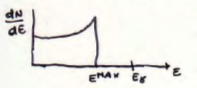
\includegraphics[scale=1]{./Immagini/SpettroCompton.png}
\caption{Spettro prodotto da un effetto Compton}
\label{fig:spettroCompton}
\end{center}
\end{figure}
\section{Produzione di coppie}
\`E il fenomeno dominante per alte energie, la coppia generata rilascia energia cinetica nel materiale e successivamente osserviamo l'annicilazione del positrone con
un elettrone.
Supponendo che tutta l'energia cinetica venga misurata posso osservare 3 picchi diversi a seconda dei fotoni da 511 keV assorbiti (figura~\ref{fig:spettroCoppia}.
\begin{figure}[htbp]
\begin{center}
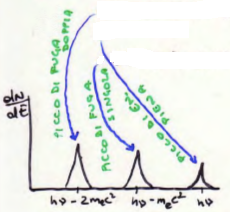
\includegraphics[scale=1]{./Immagini/SpettroCoppia.png}
\caption{Spettro prodotto dalla produzione di coppie}
\label{fig:spettroCoppia}
\end{center}
\end{figure}
Nel caso entrambi i fotoni da 511 keV vengano misurati allora osserviamo il \textbf{picco di energia piena}, tuttavia pu\`o accadere che uno dei due fotoni (o entrambi)
fuggano dal rivelatore, in questo caso osserviamo il \textbf{picco di fuga singola o doppia}.
Posso anche osservare casi intermedi, come degli effetti Compton e una successiva fuga.
\section{Funzione di risposta degli spettrometri $\gamma$}
\subsection{Caso del rivelatore piccolo}
Un rivelatore piccolo \`e un rivelatore sufficientemente grande da assorbire tutta l'energia cinetica degli elettroni, tuttavia di dimensioni inferiori al libero cammino
medio dei fotoni (che quindi non vengono, per la maggior parte, rivelati).
Lo spettro prodotto da un rivelatore di questo tipo \`e dato dal continuo del Compton, dal picco prodotto dall'effetto fotoelettrico e dal picco di doppia fuga.
\subsection{Caso del rivelatore grande}
Un rivelatore grande dovrebbe avere dimensioni nelle decine di cm, in questo caso tutti gli effetti e i fotoni secondari vengono rivelati, producendo solo 
picchi di energia piena e fotopicchi.
\subsection{Caso del rivelatore intermedio}
\`E il tipico caso di un rivelatore reale.
Posso avere picchi di energia piena insieme fughe di fotoni e scattering Compton multipli.
In questo caso la funzione di risposta del dispositivo viene simulata con metodi MonteCarlo.
Parametri importanti sono il rapporto tra il numero di picchi ad energia piena e il numero di eventi totali, il rapporto tra la fuga doppia e l'energia piena e
quello tra la fuga singola e l'energia piena.\\
La funzione di risposta di questi rivelatori ha delle complicazioni legate a:
\begin{itemize}
\item \textbf{Fuga di elettroni secondari}, che diventano importanti se il fotone \`e molto energetico o se il rivelatore \`e piccolo. Per via delle fughe l'energia misurata
	dal rivelatore sara inferiore rispetto a quella reale, peggiorando il rapporto energia piena/eventi totali.
\item \textbf{Fuga di fotoni da bremsstrahlung}, che diventa importante per elettroni molto energetici. L'energia irradiata in questo modo cresce come $Z^2$, anche in questo
	caso il continuo subisce un abbassamento di energia, oltre ad una distorsione nella forma.
\item \textbf{Fuga di raggi X caratteristici}, questo fenomeno diventa importante per fotoni ad energia minore (per via delle emissioni a cascata del fotoelettrico) e nei rivelatori con superfici
	molto pi\`u grandi rispetto al volume.
	Questo effetto produce dei picchi di fuga evidenti, in quanto i raggi X emessi hanno frequenze ben definite dai livelli energetici atomici.
\item \textbf{Radiazione secondaria prodotta vicino alla sorgente}, come la produzione di fotoni di annichilazione nell'ambiente in seguito ad un decadimento $\beta^+$.
	In questo caso viene osservato un picco a 511 keV (o a 1022 keV se il rivelatore \`e a pozzetto).
	Un altro effetto dovuto all'interazione con l'ambiente \`e la produzione di bremsstrahlung nei decadimenti $\beta^-$: in questo caso il continuo subisce un abbassamento in energia.
\item \textbf{Effetti dovuti a materiali esterni}, la radiazione prodotta dalla sorgente pu\`o interagire con l'ambiente e successivamente entrare nel rivelatore.
	Ad esempio un fotone potrebbe fare dello scattering Compton con l'ambiente e successivamente entrare nel dispositivo, in questo caso vedr\`o un aumento degli eventi nella
	regione a bassa energia. Un'altra possibilit\`a \`e un annichilazione con l'ambiente esterno, oppure la produzione di raggi X nell'ambiente esterno.
\item \textbf{Effetti dovuti alla somma di impulsi}, avviene nel caso di rate troppo intensi o nel caso di coincidenze, in questo caso il rivelatore non risolve
	temporalmente gli eventi e considera come un unico evento degli eventi distinti (\textit{pile-up}).
	In questo caso il rivelatore misurer\`a la somma delle energie e il conteggio degli eventi risulter\`a inevitabilmente falsato.
\end{itemize}
\begin{figure}[htbp]
\begin{center}
	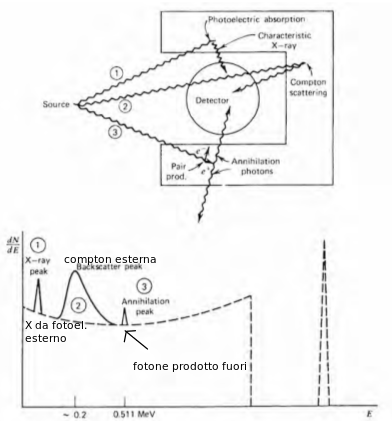
\includegraphics[scale=1]{./Immagini/EffettiGamma.png}
\caption{Possibili interazioni con l'ambiente che disturbano la misura}
\end{center}
\end{figure}
\section{Utilizzo di scintillatori come spettrometri $\gamma$}
La funzione di risposta degli scintillatori dipende dal tipo di cristallo usato, ad esempio il NaI ha un'ottima risoluzione e sezione d'urto
per effetto fotoelettrico, mentre il BGO (Bismuto-Germanio-Ossigeno) ha una sezione d'urto per fotoelettrico migliore (per cui ho meno picchi di fuga), 
ma una risoluzione peggiore in quanto ha un basso fattore di conversione energia-luce.\\
\begin{figure}[htbp]
\begin{center}
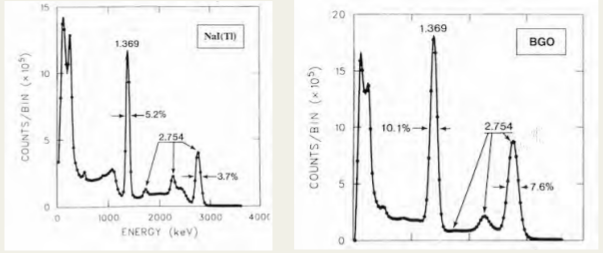
\includegraphics[scale=0.7]{./Immagini/ConfrontoRisposta.png}
\caption{Confronto delle funzioni di risposta dei due scintillatori.}
\end{center}
\end{figure}
La risoluzione \`e fondamentale per riconoscere picchi in quanto risoluzioni troppo basse potrebbero nascondere i picchi nel fondo.
\subsection{Risposta ai fotoni ad alta energia}
Quando l'energia dei fotoni aumenta (2-20 MeV), la sezione d'urto della produzione di coppie cresce.
Questo significa che verr\`a prodotta una coppia elettrone-positrone ad alta energia, quindi con una sezione d'urto per
bremsstrahlung maggiore.
Questo implica una maggiore perdit\`a alle superfici, per questo motivo all'aumentare dell'energia il picco di energia piena inizia a diminuire.
Inoltre, aumentando l'energia aumenta il numero di fotoelettroni che vengono prodotti nello scintillatore, poich\`e
FWHM $\propto N$ i picchi di energia piena, fuga singola e fuga doppia si allargano (figura~\ref{fig:confrontoAlteEnergie}).
\begin{figure}[htbp]
\begin{center}
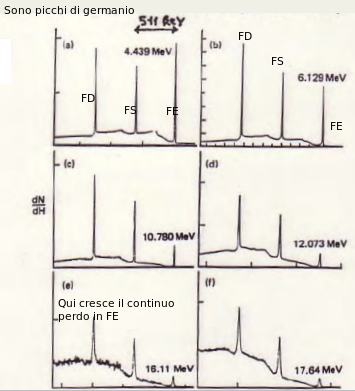
\includegraphics[scale=1]{./Immagini/ConfrontoAlteEnergie.png}
\caption{Spettro prodotto da germanio all'aumentare dell'energia}
\label{fig:confrontoAlteEnergie}
\end{center}
\end{figure}
\subsection{Linearit\`a della misura}
La relazione $L = S \cdot E$ deve essere il pi\`u possibile lineare, in quanto misuro con punti discreti, quindi devo
avere meno errori legati alla discretizzazione di una funzione continua.
La linearit\`a dipende dal tipo di particella e dall'energia: per elettroni la relazione ha una non-linearit\`a piuttosto ridotta;
per i fotoni, poich\`e la sequenza di interazioni che esso fa \`e diversa per ogni fotone che viene rivelato, esiste una maggiore
variabilit\`a, quindi le fluttuazioni sono maggiori, tuttavia comunque mantiene una certa linearit\`a per via del fatto che viene
misurato mediante interazioni con elettroni.
\begin{figure}[htbp]
\begin{center}
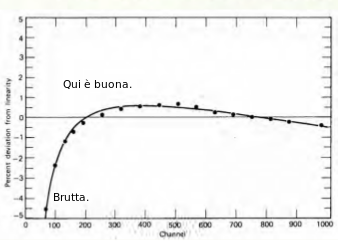
\includegraphics[scale=1.00]{./Immagini/LinearitaScintillatore.png}
\caption{Percentuale di deviazione dalla linearit\`a per uno scintillatore. Esiste un range dove essa \`e rispettata.}
\end{center}
\end{figure}
\subsection{Calibrazione in energia dei rivelatori}
Per calibrare i rivelatori si usano delle sorgenti ad energie note, in generale si cerca di usare dei $\gamma$ con energie ben spaziate
su tutto il range energetico di interesse.
I raggi $\gamma$ sono noti con una precisione energetica di $10^{-5}$, per questo \`e importante utilizzare sorgenti note con quella
precisione, per questo motivo esistono delle sorgenti standard di calibrazione:
\begin{itemize}
\item K$_{\alpha}$(W) (tungsteno) a 5.9 keV
\item $^{198}$Au a 412 keV
\item $^{60}$Co a 1333 keV
\end{itemize}
\textbf{Non si possono usare i fotoni di annichilazione} in quanto il decadimento non avviene sempre a riposo.\\
Inoltre se ho una fuga singola o doppia in una regione ben calibrata, posso usarla per controllare la correttezza della calibrazione,
lo stesso vale nel caso dell'emissione in cascata di fotoni.\\
La curva di calibrazione viene ottenuta interpolando i punti con una funzione polinomiale del tipo
\begin{equation*}
E_i = \sum_{n=0}^N a_n C_i^n
\end{equation*}
con $N \approx 4-5$ utilizzando il metodo dei minimi quadrati.\\
Sono state osservate dipendenze dalla direzione di incidenza della radiazione della risposta, per questo motivo \`e necessario calibrare
tenendo conto del lato che verr\`a esposto alla radiazione. 
Queste variazioni sono nell'ordine dei 100 eV, per questo motivo diventano importanti per misure molto precise;
questo accade perch\`e il campo elettrico degli elettroni influisce sulla raccolta dei fotoni.
\subsection{Convenzioni sulle efficienze nella spettroscopia $\gamma$}
Alcuni rapporti sono molto diffusi nella descrizione delle efficienze dei rivelatori:
\begin{itemize}
\item \textbf{Rapporto picco-Compton}, viene definita sul decadimento del $^{137}$Cs  a 662 keV come:
\begin{equation*}
R_{pc} = \frac{\text{Conteggi/canale al canale del massimo}}{\text{Conteggi/canale medi nella regione tra 358 e 382 keV}}
\end{equation*}
oppure sul decadimento del $^{60}$Co a 1333 keV:
\begin{equation*}
R_{pc} = \frac{\text{Conteggi/canale al canale del massimo}}{\text{Conteggi/canale medi nella regione tra 1040 e 1096 keV}}
\end{equation*}
Gli intervalli di energia sono stati scelti in quanto in quella regione non \`e presente radiazione naturale, ma solamente Compton.
Questo parametro serve a dare una misura combinata della FWHM con la fotofrazione $R_{ph}$:
\begin{equation*}
R_{ph} = \frac{\text{Area del picco ad energia piena}}{\text{Area totale dello spettro}}
\end{equation*}
$R_{pc}$ viene peggiorato dallo scattering Compton con l'ambiente.
A parit\`a di fotofrazione si osserva che $R_{pc} \propto \frac{1}{\text{FWHM}}$ e, a parit\`a di FWHM, $R_{pc} \propto R_{ph}$ (\textbf{perch\`e?}).
\item \textbf{Efficienza assoluta del picco ad energia piena} $\epsilon_{ap}$
\item \textbf{Efficienza intrinseca del picco ad energia piena} $\epsilon_{ip}$, tipicamente viene quotato per $^60$Co a 1333 keV
\item \textbf{Volume attivo}, ad alte energie $\epsilon_{ip} \propto V_{att}$
\item \textbf{Efficienza relativa}, a volte l'efficienza viene quotata rispetto all'efficienza di un rivelatore a NaI di $3''\times 3''$ 
con sorgente di $^{60}$Co posta a 25 cm di distanza con fotoni a 1333 keV, questa efficienza vale $\epsilon_{ap} = 1.2 \cdot 10^{-3}$
\item \textbf{Regola del pollice}, poich\`e l'efficienza ha una dipendenza dal volume, a volte viene data per unit\`a di volume, ad esempio per il germanio (rivelatore HPGe) vale:
\begin{equation*}
\epsilon_{rel}^{Ge} \approx \frac{V[\text{cm}^3]}{5}\%
\end{equation*}
Per cui un germanio al 100\% ha un volume di 500 cm$^3$.
\end{itemize}